% Please use the skeleton file you have received in the
% invitation-to-submit email, where your data are already
% filled in. Otherwise please make sure you insert your
% data according to the instructions in PoSauthmanual.pdf
\documentclass{PoS}

\title{Search for Neutrinos from Populations of Optical Transients}

\ShortTitle{Neutrinos from Optical Transient Populations}

\author{
The IceCube Collaboration$^{\dagger}$\\
{$^{\dagger}$ \itshape \href{http://icecube.wisc.edu/collaboration/authors/icrc19_icecube}{http://icecube.wisc.edu/collaboration/authors/icrc19\_icecube}}\\
E-mail: \email{robert.stein@desy.de}
}

\usepackage{lineno}
\linenumbers

\abstract{

Since the detection of high-energy cosmic neutrinos at the IceCube Neutrino Observatory in 2013, there has been an on-going search to find suitable transient or variable source candidates. Despite recent evidence identifying a flaring blazar as a possible neutrino source, the vast majority of the diffuse neutrino flux measured by IceCube remains unexplained. The latest IceCube results testing time-dependent correlation between neutrinos and Tidal Disruption Events (TDEs) are presented, limiting the contribution of jetted and non-jetted TDEs of the diffuse astrophysical neutrino flux to be less than 1.3\% and 26\% respectively. In addition, a dedicated search for neutrinos from the extraordinary transient AT2018cow are presented, and upper limits on the integrated neutrino emission are derived. Expected improvements from new and upcoming time domain optical surveys (such as ZTF and LSST) are also introduced.\\

% comment the following section if you use analysis@icecube.wisc.edu
\vspace{4mm}
{\bfseries Corresponding authors:}
\speaker{Robert Stein}$^{1}$\\
{$^{1}$ \itshape DESY Zeuthen, Platanenallee 6, 15738 Zeuthen, Germany}\\

%end comment

}

\FullConference{36th International Cosmic Ray Conference -ICRC2019-\\
		July 24th - August 1st, 2019\\
		Madison, WI, U.S.A.}


\begin{document}
	
\section{Introduction}

The IceCube Neutrino Observatory is a cubic-kilometer array buried 1.5 km beneath glacier ice at the geographic south pole \cite{Aartsen:2016nxy}. When neutrinos undergo charged-current  or neutral-current interactions in the ice, daughter leptons emit Cherenkov light that can be detected by IceCube's 5160 Detector Optical Modules (DOMs). In 2013, IceCube discovered a diffuse flux of high-energy astrophysical neutrinos \cite{Aartsen:2013jdh}, and there has since been an ongoing search to find potential source candidates. Auto-correlation analyses searching for steady neutrino sources, neutrino flares or coincident neutrino multiplets have so far failed to find any significant clustering within the neutrino flux (e.g  \cite{Aartsen:2016oji}). The consistency of this flux with an isotropic distribution suggests that it has a predominantly extragalactic origin. The lack of independently-identified neutrino sources has motivated targeted searches using multi-wavelength and multi-messenger data, seeking to identify an excess of neutrinos correlated with a given source or source class. In general, the sensitivity of neutrino telescopes is limited by the background flux of atmospheric neutrinos, as well as atmospheric muons, which exceed the measured astrophysical neutrino flux by orders of magnitude except at the very highest energies above O(100TeV). 

This vast background can be overcome with two complementary approaches. In the neutrino-driven approach, neutrino events are selected which have a high-probability to be of astrophysical orgin, based on their reconstructed topology. For these neutrinos, possible counterparts can be identified. Such an approach forms the basis of the IceCube Realtime Program, in which likely astrophysical neutrinos are identified in real-time and immediately distributed as "alerts" to astronomers via the Gamma-ray Coordination Network (GCN) framework \cite{Aartsen:2016lmt}. Because only a handful of neutrinos are identified with these filters each year, it can be hard to make statistically-signficant statements about source populations using this approach. Furthermore, these searches are hampered by the abundance of undetected neutrino sources that would be expected for most source populations. For the case of a CCSN-like population of neutrino sources, just 20\% of all astrophysical neutrinos would be expected to have detectable counterparts \cite{Kankare:2019bzi}, assuming that they were followed up by the most sensitive current instruments.

In the alternative source-driven approach, specific source hypotheses are tested. These searches typically exploit the large expected number of lower-energy astrophysical neutrinos, enabling analysis with significantly higher statistics at the cost of greater atmospheric background \cite{Aartsen:2016oji}. Requiring spatial coincidence with a potential source does, however, significantly reduce the background for a search. Another effective method is to additionally require temporal coincidence, either with the lifetime of a transient, or during  pre-defined "interesting periods" for variable objects. Multiple sources can be combined in a stacking analysis, which are designed to detect the sum of many weak individual sources. In all cases, these methods rely on multi-messenger and multi-wavelength observations to identify sources to be analysed.

The most sucessful example of the neutrino-driven approach followed the detection of a high-energy neutrino  IC170922A, following which a comprehensive multi-messenger follow-up campaign was launched \cite{IceCube:2018dnn}. The Fermi collaboration reported that the neutrino was coincident with a flaring gamma-ray blazar. A chance coincidence of this kind was disfavoured at the level of 3$\sigma$. At the same time, previous IceCube analysis has limited the cumulative distribution of Fermi blazars to the astrophysical neutrino flux to be less than 30\% \cite{Aartsen:2016lir}. The origin of the vast majority of the diffuse neutrino flux thus remains, as yet, undiscovered. Dedicated searches targeting likely sources, including Gamma-Ray Bursts (GRBs), Core-Collapse Supernovae (CCSNe), Starburst galaxies and galactic emission, have so far failed to reveal any significant excess above background expectations \cite{Stasik2018Search}. This motivates the continued analysis of new, untested source classes in an attempt to identify the origin of astrophysical neutrinos.

\section{Tidal Disruption Events}

Within this context, a new analysis was undertaken to search for neutrinos from Tidal Disruption Events (TDEs). A TDE occurs when a star approaches a supermassive black hole (SMBH) on a parabolic orbit \cite{Komossa:2015qya}. As gravitational acceleration follows a $\frac{1}{r^{2}}$ dependence, the near side of the star will be accelerated more strongly than the far side. The star thus experiences a net tidal force. As the star moves closer to the SMBH, the tidal force increases, until it exceeds the self-gravity that holds the star together. At this point, the star is said to be tidally-disrupted, and roughly half of the stellar debris is accreted. In some cases, a relativistic jet can be formed during the accretion process, analagously to a blazar jet. There has been recent theoretical interest in TDEs as potential Ulta-High Energy Cosmic Ray (UHECR) sources, as well as candidate neutrino sources (e.g \cite{Biehl:2017hnb}).

TDEs are a fundamentally rare phemomenon, with rates several orders of magnitude below CCSN rates \cite{vanVelzen:2017qum}. However, historically poor detection efficiences have further exacerbated this, leaving only a handful of reliably-identified TDEs. To date, there have been only 3 on-axis jetted TDEs, and a few dozen candidate non-jetted TDEs \cite{Komossa:2015qya, Auchettl:2016qfa}. Of these, the majority do not have an unambiguous TDE classification. 

TDEs themselves are, by their nature, nuclear transients. They can often be confused with flares of Active Galactic Nuclei (AGN), as well as nuclear CCSNe. Due to the greater abundance of these background populations, it can be hard to remove all contamination. Ultimately muliple eras of spectroscopy and photometry are required for a compelling classification. At the time of catalogue compilation in October 2017 \cite{Auchettl:2016qfa}, out of approximately 60 candidate TDEs in the literature overlapping IceCube data-taking, only 13 were judged to be unambigouously classified. 

\section{Results}
\subsection{Stacking Search}

The stacking method employed for the analysis did not make assumptions on the relative strength of each tested source, and was thus robust against both catalogue contamination and deviations from a standard-candle neutrino emission scheme \cite{Stasik2018Search}. However, in order to meaningfully interpret the results, and extrapolate to constrain emission from the population as a whole, a pure sample is required. 

\begin{figure}[!ht]
	\centering 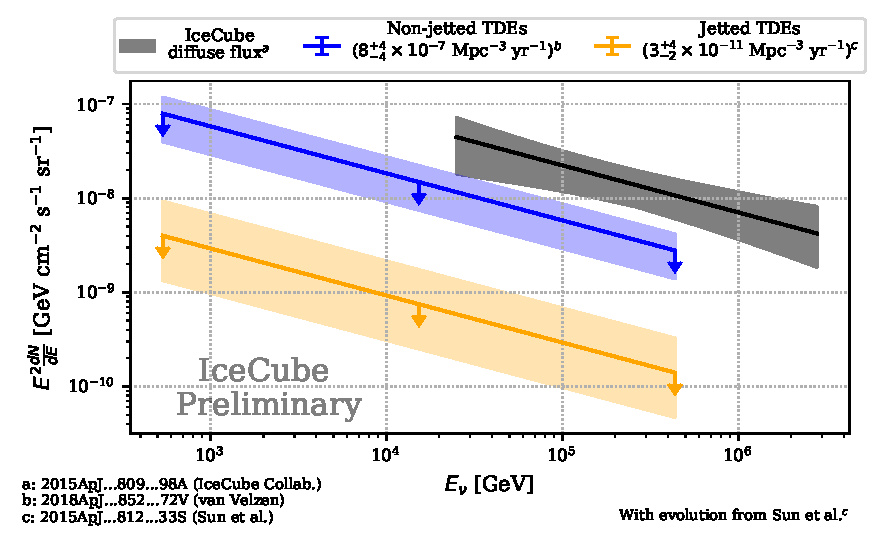
\includegraphics[width=\textwidth]{figures/diffuse_flux_global_fit}
	\caption{Limits on the contribution of jetted and non-jetted TDEs to the diffuse neutrino flux. The shaded bands represent unceratinty in local rate estimates.}
	\label{fig:DiffuseFlux}
\end{figure}

Consequently, the non-jetted sample was separated based on robustness of classification. A "golden sample" of unambiguous TDEs was created, and a speparate "silver sample" of likely TDEs was also created. A third category of "obscured TDEs" was also created, for TDE candidates from XYZ that were found to in dusty galaxies. As these obscured TDEs were detected only via Infra-red observation, for which we expect significant reprocessing, there would likely be a variable time lag between the disruption itself and the corresponding IR flare. As we expect that neutrinos should generally arrive after the disruption, these obscured TDEs were treated with larger, more conservative search windows to account for this additional uncertainty. These three categories do not form physically distinct classes, but rather differing levels of observational data and likely contamination.

For each source, a tailored search window was defined, with the aim of covering the period from 30 days before peak to 100 days after. This specific choice was motivated by the range of theoretical predictions for TDE neutrino emission, all of which broadly agree that emission should coincide with the operiod of peak EM brightness following the disruption. Due to the sparsity of available observational data, this search window was conservatively extended for sources without a resolved lightcurve peak, extending to the last available upper limit. In cases where no upper limit was available, the window was instead set to be one year before observed peak up to 100 days afterwards. With this method, there is reasonable certainty that the lightcurve peak fell within the search window for each TDE. For the obscured TDEs, accounting for time lags that were expected to be roughly of order 100 days, all windows were fixed to extend from one year before IR lightcurve peak, to 100 days after peak.

With each of the four catalogues, an independent test for neutrino correlation was performed. In all cases, the results were consistent with expectations from background, and thus upper limits are accordingly derived. Separate upper limits were derived for the two distinct source populations, namely on-axis jettted TDEs and non-jetted TDEs. For the calculation of these source population limits, the "Golden TDEs" were assumed to be representative of non-jetted TDEs as a whole. 

By assuing that these TDEs behave as standard candles, per-source limits on neutrino emission can be derived.  The results are shown in Figure \ref{fig:DiffuseFlux}. Assuming central rate estimates from \cite{vanVelzen:2017qum} and \cite{Sun:2015bda}, we find that non-jetted and jetted TDEs contribute less than 26\% and 1.3\% respectively to the astrophysical neutrino flux. As the contribution from a population is directly proportional to the local population rate, the shaded bands indicate the uncertainty in our limits arising from rate estimates. For TDEs, these rates are the dominant source of uncertainty in neutrino flux. It will require systematic evaluation of observed TDE rates to enable more precise limits on neutrino emission. Any refined rate estimate can be immediatly used to diretly recalculate  limits, without requiring any additional IceCube analysis.

\subsection{AT2018cow}

The discovery of extraordinary transient AT2018cow was a further demonstration of the central importance of multi-messenger observations.  This fast, bright, blue transient prompted a comprehensive multi-messenger follow-up campaign, and was variously interpreted as a TDE, an extreme SN or a Magnetar \cite{Perley:2018oky}. The observations were consistent with a nearby example of a recently-identified population of Fast Blue Optical Transients (FBOTs). A new analysis of AT2018cow, extending from 30 days before peak to 100 days afterwards, did not reveal any significant neutrino emission. The corresponding constraints are illustrated in Figure \ref{fig:At2018cow}. As before, uncertainty in both classification and rate estimates hinder attempts to constrain neutrino emission from FBOTs.

\begin{figure}[!ht]
	\centering 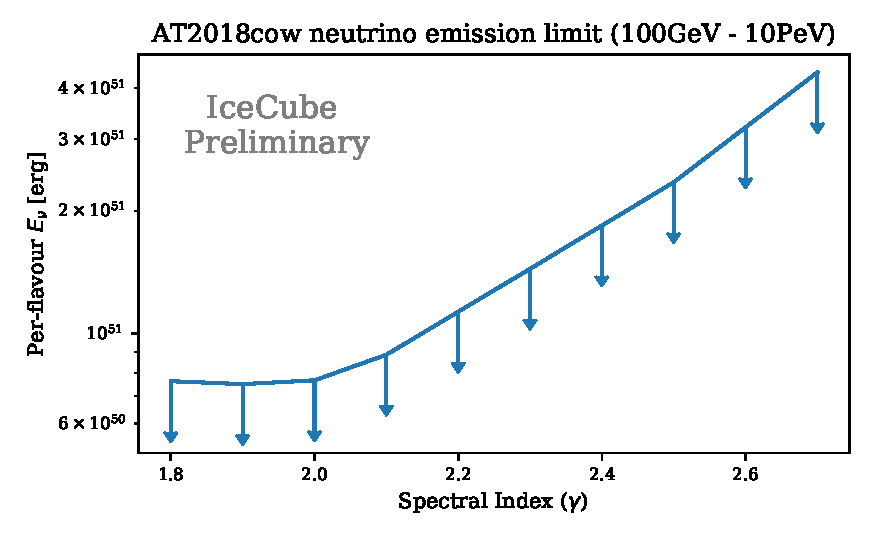
\includegraphics[width=.9\textwidth]{figures/AT2018cow_limit_plot}
	\caption{Limits on integrated neutrino emission from AT2018cow as a function of spectral index, assuming a 130 day window from MJD 58256.9 to MJD 58386.9}
	\label{fig:At2018cow}
\end{figure}

\section{Outlook}

Fortunately, the emergence of new facilities such as ZTF, as well as future surveys such as LSST, should greatly aid such analyses. By discovering larger numbers of transients, the sensitivity of searches will grow. Larger samples should also improve rate estimation. Higher cadence observations can greatly reduce background by constraining search windows, for example the estimated CCSN explosion time, with greater precision. Consequently, source-driven analysis will continue to grow more powerful.

\bibliographystyle{ICRC}
\bibliography{my-bib-database}

% Or, set up the bibliography manually, if you prefer to do things this way.
%
% \begin{thebibliography}{99}
%   \bibitem{Zoll:2015wcu}{{\bf IceCube} Collaboration, \pos{PoS(ICRC2015)1099} (2016).}
%   \bibitem{Peiffer:2017vsm}{{\bf IceCube-Gen2} Collaboration, \pos{PoS(ICRC2017)1052} (2018).}
%   \bibitem{Hussain:2019icrc_gw}{{\bf IceCube} Collaboration, \pos{PoS(ICRC2019)xyz} (these proceedings).}
%   \bibitem{Aartsen:2016nxy}{{\bf IceCube} Collaboration, M.~G.~Aartsen {et al.}, \emph{JINST} {\bf 12} (2017) P03012%
%   % optionally add arXiv ID here [{\tt astro-ph/1612.05093}]
%   .}
%   \bibitem{Waxman:1998yy}{E. Waxman and J. N. Bahcall, \emph{Phys. Rev.} {\bf D59} (1999) 023002.}
% \end{thebibliography}

\end{document}
